\section{Phương pháp}

\subsection{Dữ liệu}
\begin{frame}{\secname: \subsecname}
\begin{enumerate}
    \item QaTa-COV19-v2: bao gồm 9258 ảnh X-ray ngực được ghi chú thủ công thương tổn do COVID-19 lần đầu tiên. Nhóm nghiên cứu đã mở rộng ghi chú với sự hỗ trợ của các chuyên gia. Ghi chú tập trung vào cả hai phổi có nhiễm bệnh, số vùng thương tổn, vị trí tương đối của vùng nhiễm bệnh. Ví dụ: "Bilateral pulmonary infection, two infected areas, upper left lung and upper right lung" (tạm dịch: "Cả hai phổi bị nhiễm bệnh, hai vùng bị nhiễm, phía trên phổi trái và phía trên phổi phải").
    % \item MosMesData+ \footnotemark: bao gồm 2729 ảnh CT scan về nhiễm trùng phổi. Ghi chú của tập dữ liệu có cấu trúc tương tự QaTa-COV19. Ví dụ: "Unilateral pulmonary infection, two infected areas, middle lower left lung" (tạm dịch: "Một bên phổi bị nhiễm bệnh, hai vùng bị nhiễm, ở giữa phía dưới phổi trái").
    \item MosMesData+: bao gồm 2729 ảnh CT scan về nhiễm trùng phổi. Ghi chú của tập dữ liệu có cấu trúc tương tự QaTa-COV19. Ví dụ: "Unilateral pulmonary infection, two infected areas, middle lower left lung" (tạm dịch: "Một bên phổi bị nhiễm bệnh, hai vùng bị nhiễm, ở giữa phía dưới phổi trái").
    \item ESO-CT: bao gồm 286 ảnh X-ray được ghi chú độc lập bởi hai chuyên gia.
\end{enumerate}
    % \footnotetext[1]{\href{http://medicalsegmentation.com/covid19}{http://medicalsegmentation.com/covid19}}
\end{frame}

\begin{frame}{\secname: \subsecname}
Cụ thể, số lượng mẫu được chia trong từng tập như sau:

\begin{table}[H]
    \centering
    \begin{tabular}{cccc}
    \hline
    & \textbf{QaTa-COV19-v2} & \textbf{MosMedData+} & \textbf{ESO-CT} \\
    \hline
    Tập huấn luyện & 5716 & 2183 & 182 \\
    Tập kiểm định & 1429 & 273 & 273 \\
    Tập kiểm thử & 2113 & 273 & 58 \\
    \hline
    Tổng cộng & 9528 & 2729 & 286 \\
    \hline
    \end{tabular}
    \caption{Phân phối dữ liệu trong các tập dữ liệu}
\end{table}

\end{frame}

\begin{frame}{\secname: \subsecname}
    \begin{columns}
        \begin{column}{0.4\linewidth}
            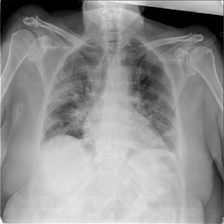
\includegraphics[width=0.6\linewidth]{images/qata-cov19-v2-covid_1.png}

            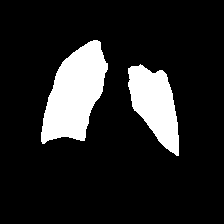
\includegraphics[width=0.6\linewidth]{images/qata-cov19-v2-mask_covid_1.png}

            QaTa-COV19-v2 (224 x 224)
        \end{column}

        \begin{column}{0.4\linewidth}
            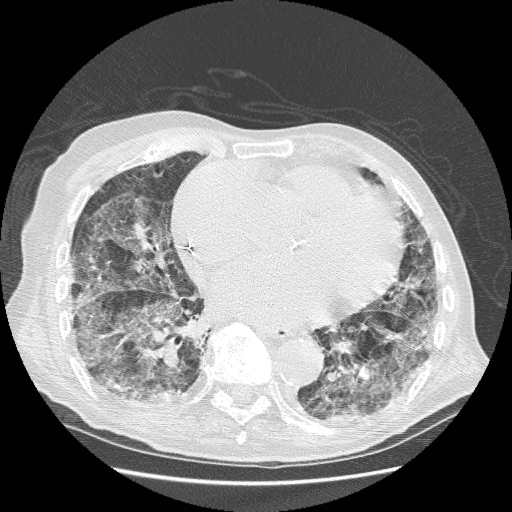
\includegraphics[width=0.6\linewidth]{images/mosmed_bjorke_1.png}

            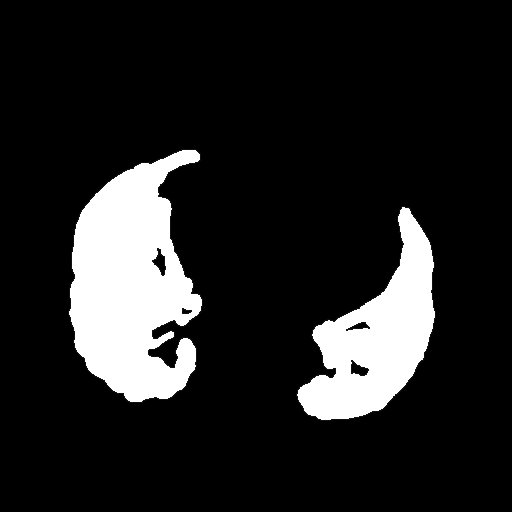
\includegraphics[width=0.6\linewidth]{images/mosmed_mask_bjorke_1.png}

            MosMedData+ (512 x 512)
        \end{column}
    \end{columns}
\end{frame}

\subsection{Quy trình xây dựng chú thích văn bản}
\begin{frame}{\secname: \subsecname}

Phần ghi chú thông tin bệnh của các bộ dữ liệu không có sẵn ngay từ đầu, mà được nhóm nghiên cứu tạo ra và mở rộng với sự hỗ trợ trực tiếp của hai chuyên gia từ Khoa Xạ trị Ung thư \footnote{Trung tâm Y tế Tây Nam trường Đại học Texas}. \\

\bigskip
Các bác sĩ X-quang tiến hành chú thích độc lập trên cùng một ảnh. Sau đó, kết quả được nhóm nghiên cứu đối chiếu để đảm bảo tính nhất quán, họ cũng kiểm tra chéo các đoạn văn bản này với mặt nạ phân đoạn gốc của ảnh nhằm bảo đảm rằng thông tin vị trí trong văn bản không sai lệch quá lớn so với vùng tổn thương thực tế.

\end{frame}


\subsection{Cấu trúc chú thích}

\begin{frame}{\secname: \subsecname}

\begin{itemize}
    \item \textbf{QaTa-COV19-v2 và MosMedData+:} Văn bản chú thích được cấu trúc hóa thống nhất, tập trung vào ba thuộc tính chính: phạm vi nhiễm bệnh, số lượng vùng tổn thương và vị trí ước chừng của vùng nhiễm.

    \item \textbf{ESO-CT:} Tập dữ liệu ung thư thực quản bao gồm các thông tin lâm sàng được bác sĩ X-quang chú thích thủ công. Để tạo văn bản mô tả, bác sĩ chia thực quản thành bốn phần từ trên xuống dưới, gồm cổ, ngực trên, ngực giữa và ngực dưới; sau đó ghi chú vị trí ước chừng của khối u dựa trên các phần này. Đoạn văn bản mô tả vị trí thô được sử dụng trực tiếp làm đầu vào cho mô hình.
\end{itemize}

\end{frame}


\begin{frame}{\secname: \subsecname}

Tập ESO-CT được đề cập trong phần phương pháp; tuy nhiên, tại thời điểm thực hiện báo cáo này, bộ dữ liệu này chưa được công bố công khai nên không thể truy cập để tiến hành thử nghiệm.

\end{frame}


\subsection{Kiến trúc mô hình}
\begin{frame}{\secname: \subsecname}
    \begin{figure}[h]
        \centering
        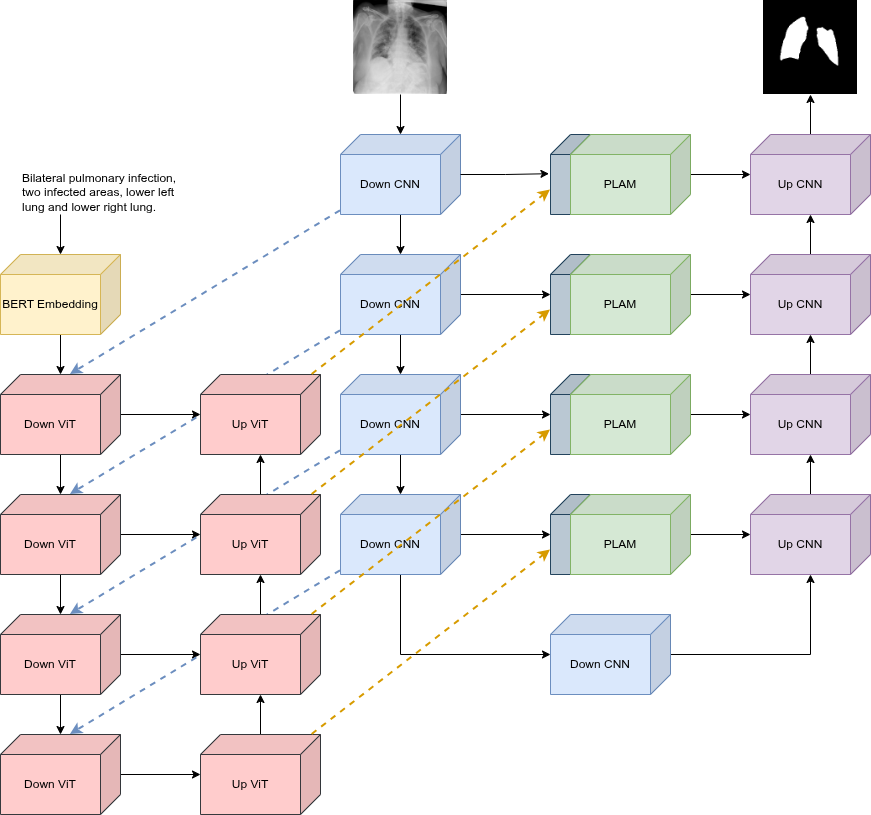
\includegraphics[width=0.6\textwidth]{images/lvit.png}
        \caption{Kiến trúc LViT.}
    \end{figure}
\end{frame}

\begin{frame}{\secname: \subsecname}
    \begin{figure}[h]
        \centering
        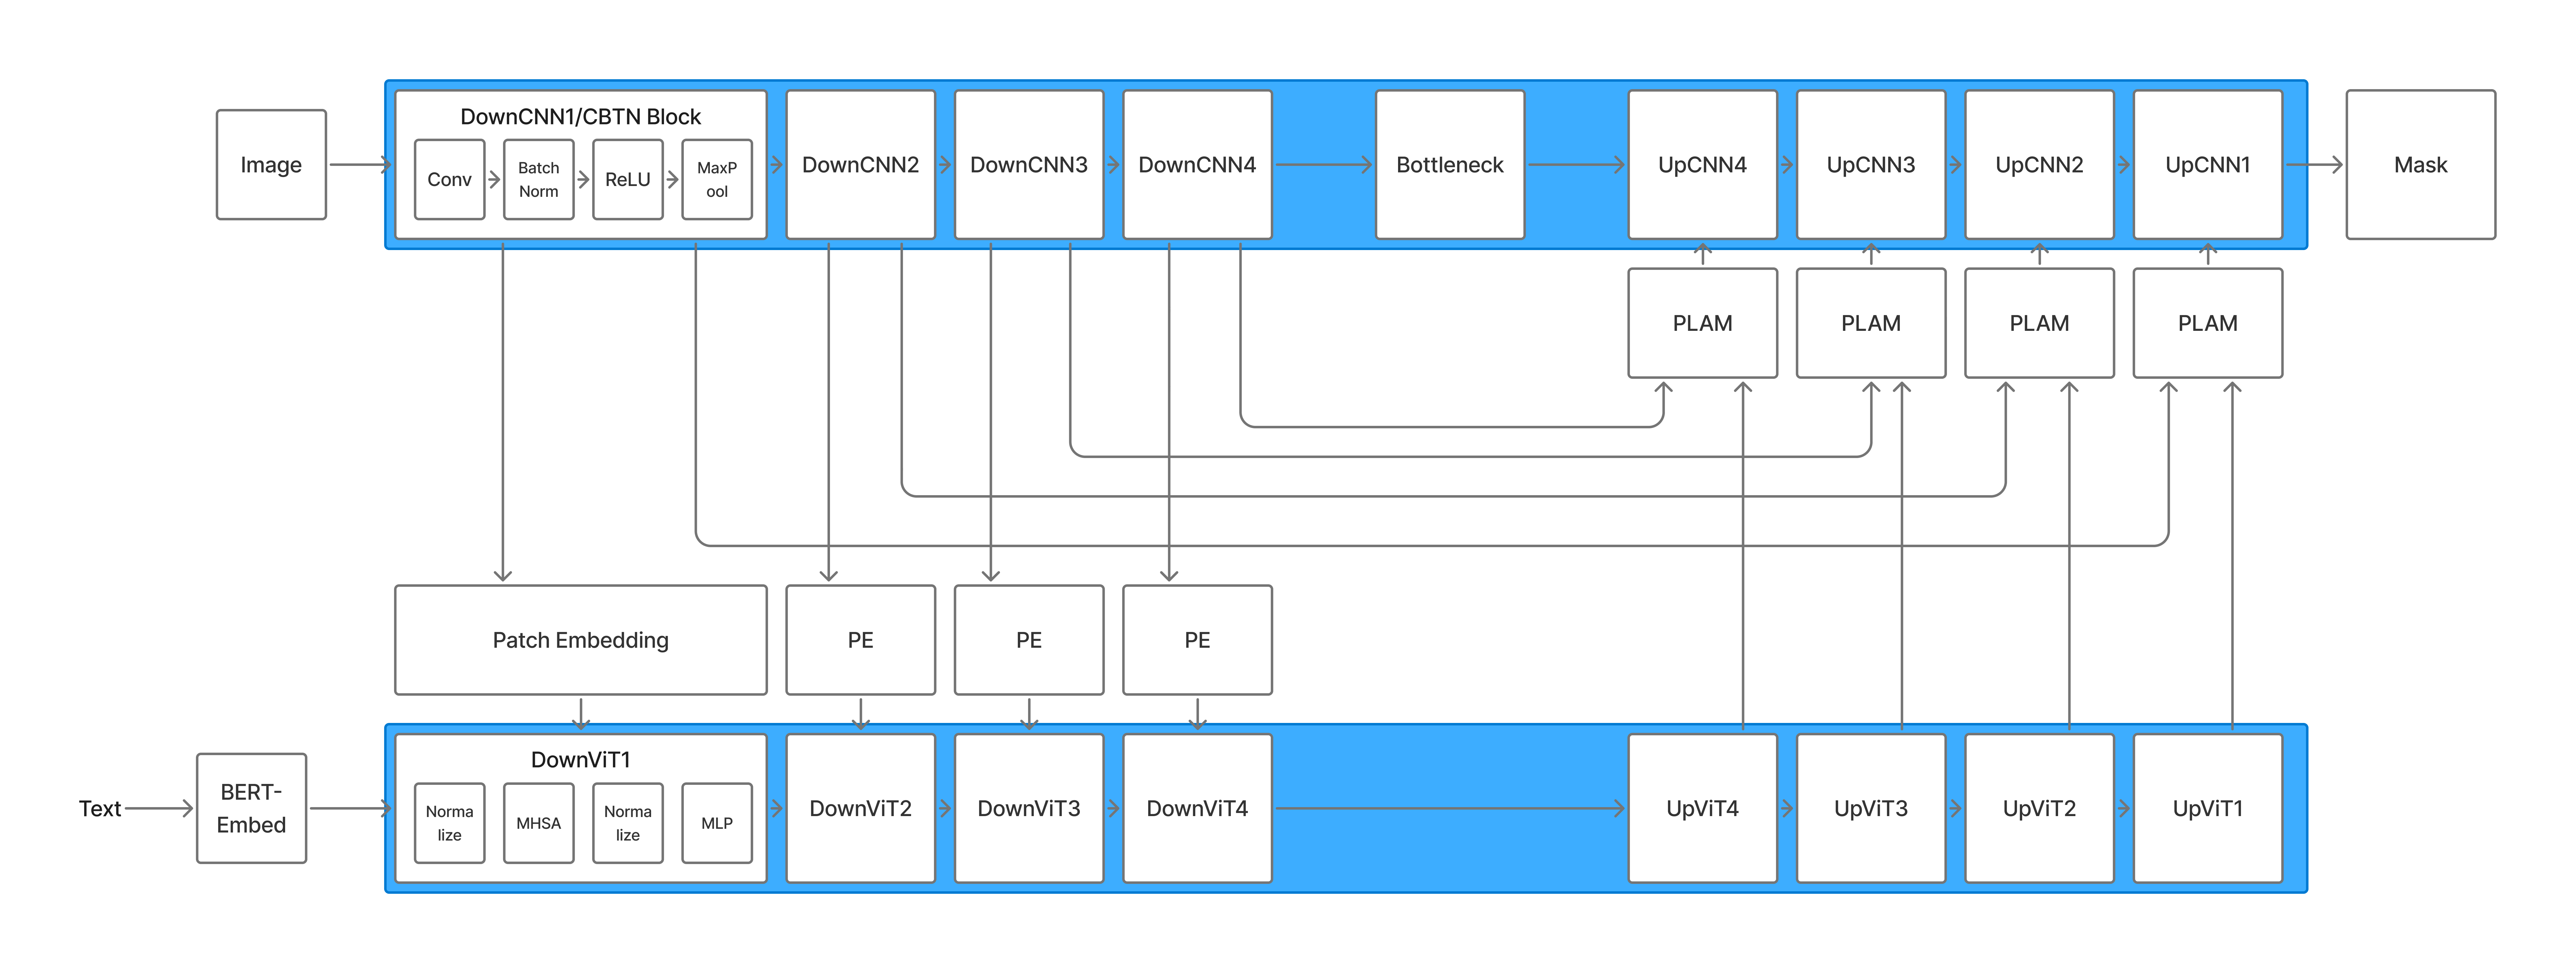
\includegraphics[width=0.8\textwidth]{images/flatten-lvit.png}
        \caption{Làm phẳng quá trình xử lý đặc trưng.}
    \end{figure}
\end{frame}

\begin{frame}{\secname: \subsecname}
\begin{enumerate}
    \item Nhánh CNN U-shape
    \item Nhánh ViT U-shape
\end{enumerate}
\end{frame}

\begin{frame}{\secname: \subsecname: CNN}
    Nhánh CNN nhận đầu vào là một ảnh và đầu ra là bản đồ xác suất.
    % CHI TIẾT CÔNG THỨC TOÁN CONVOLUTION, KÍCH THƯỚC KERNEL, ĐỘ PHÂN GIẢI SAU CNN
    \begin{columns}
        \column{0.5\linewidth}
            \begin{align*}
                D_i &= DownCNN_i = CTBN \\
                    &= ReLU(BatchNorm_i(Conv_i(\cdot)))
            \end{align*}
            \[
                Y_{DownCNN, i+1} = MaxPool(D_i(Y_{DownCNN, i}))
            \]
            \[
                Y_{DownCNN, 0} = I
            \]

        \column{0.5\linewidth}
            \hspace{0.3\linewidth}
            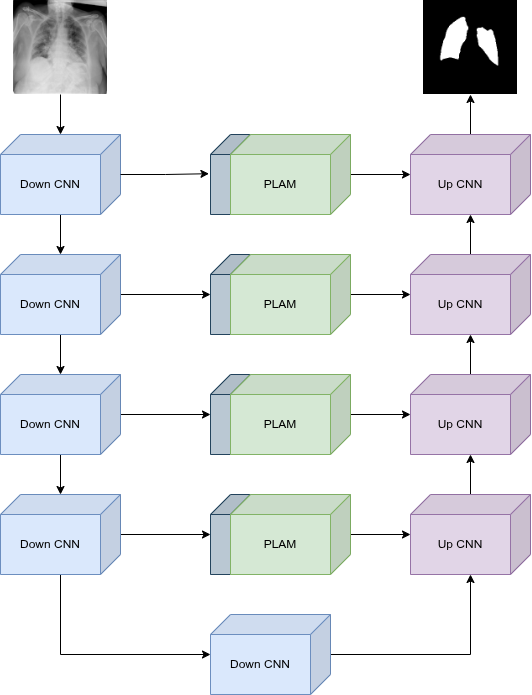
\includegraphics[width=0.6\linewidth]{images/cnn-branch.png}
    \end{columns}
\end{frame}

\begin{frame}{\secname: \subsecname: ViT}
    Nhánh ViT nhận đầu vào là đặc trưng ảnh của khối DownCNN đầu tiên cùng với đặc trưng văn bản từ lớp BERT-Embed của BERT\_12\_768\_12.
    % NÓI RÕ PATCH EMBEDDING LÀ TẠO VISUAL TOKEN
    \begin{columns}
        \column{0.4\linewidth}
            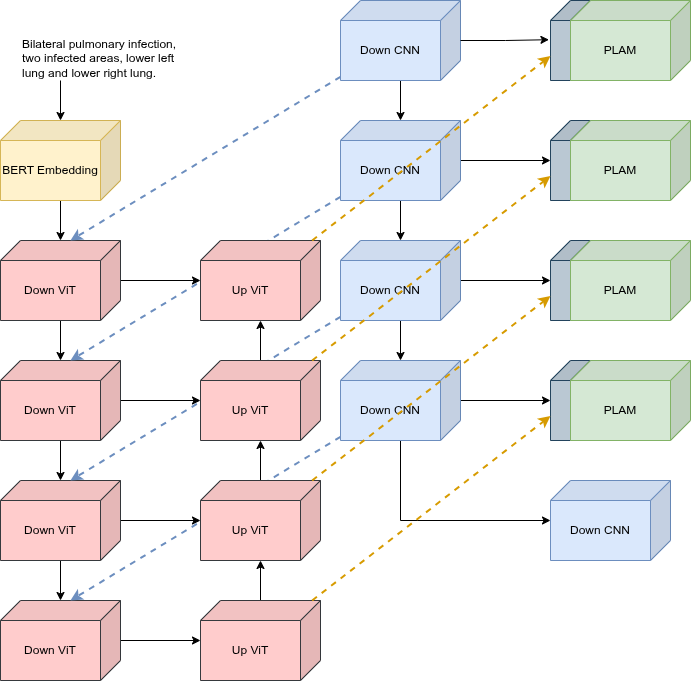
\includegraphics[width=\linewidth]{images/vit-branch.png}
        
        \column{0.6\linewidth}
            \[ViT(x) = ViT_2(ViT_1(x))\]
            \[x' = ViT_1(x) = MHSA(LN(x)) + x\]
            \[Y = ViT_2(x') = MLP(LN(x')) + x'\]
            \[x_{img, i} = PatchEmbedding(Y_{DownCNN, i})\]
            \[Y_{DownViT, 1} = ViT(x_{img, 1} + CTBN(x_{text}))\]
            \[Y_{DownViT, i+1} = ViT(Y_{DownViT, i} + x_{img, i + 1})\]

    \end{columns}
\end{frame}

\begin{frame}{\secname: \subsecname: BERT}
    \begin{figure}[h]
        \centering
        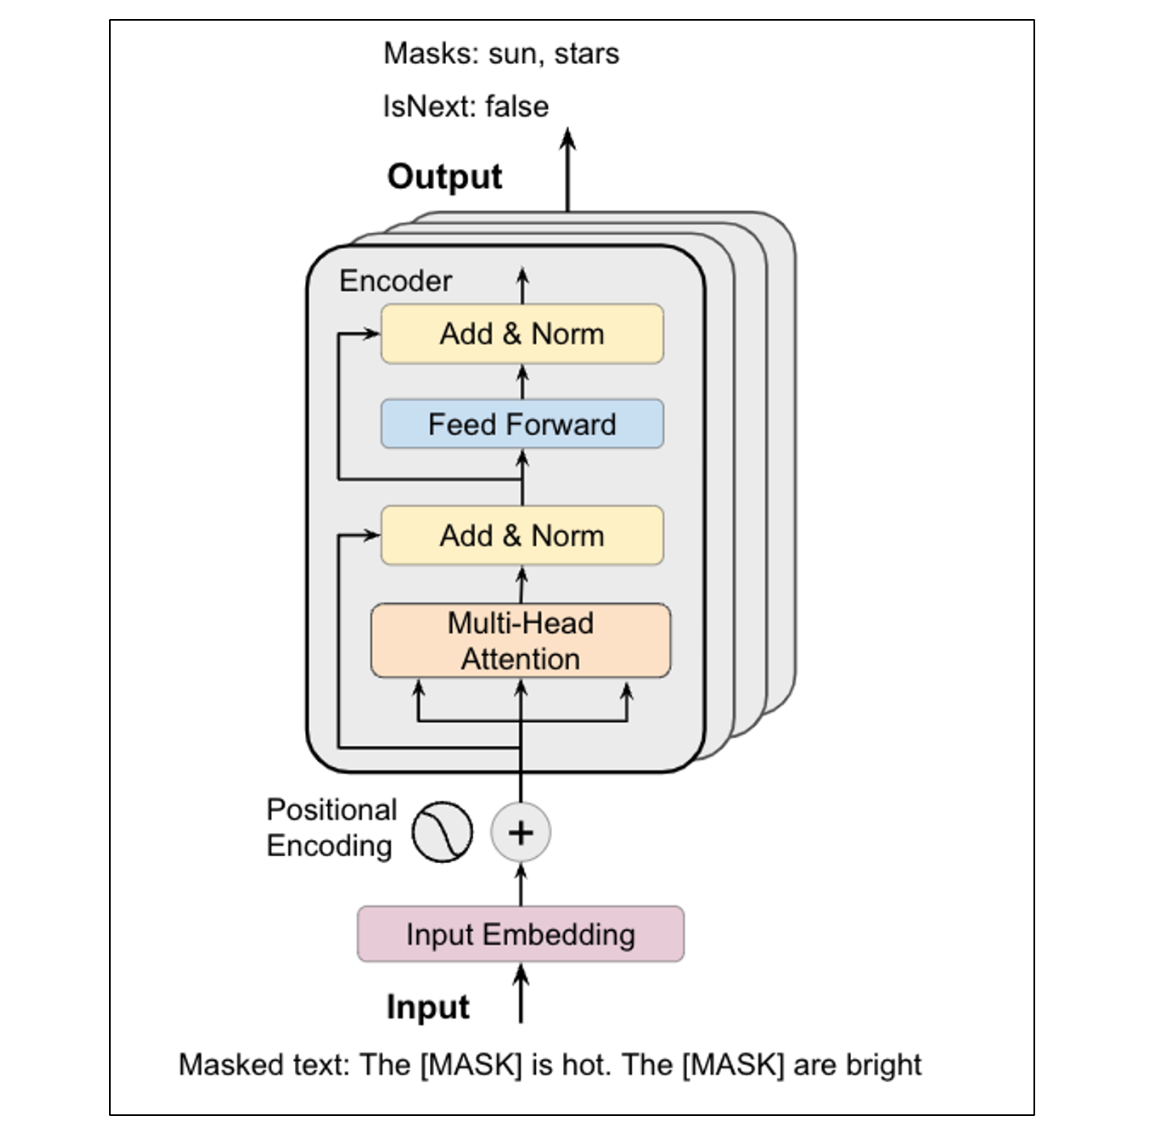
\includegraphics[height=0.7\textheight]{images/bert.png}
        \caption{Bộ mã hoá văn bản dựa trên BERT.}
    \end{figure}
\end{frame}

\begin{frame}{\secname: \subsecname: BERT}

    Trong LViT, các câu mô tả y khoa thường có cấu trúc tương đối cố định và ngắn gọn, ví dụ bao gồm phạm vi nhiễm bệnh, số vùng tổn thương và vị trí tương đối. Do đó, mô hình không nhất thiết phải sử dụng toàn bộ các tầng Transformer của BERT để suy luận ngữ cảnh phức tạp như trong các bài toán xử lý ngôn ngữ tự nhiên tổng quát. Thay vào đó, việc sử dụng lớp Embedding của BERT đã đủ để cung cấp biểu diễn ban đầu cho các token văn bản, đồng thời giúp giảm số lượng tham số, tiết kiệm chi phí tính toán và hạn chế nguy cơ quá khớp khi dữ liệu y khoa có quy mô không quá lớn.

\end{frame}


\begin{frame}{\secname: \subsecname: PatchEmbedding}

    Để kết hợp đặc trưng thị giác từ ảnh với đặc trưng văn bản trong nhánh Transformer, bản đồ đặc trưng hình ảnh cần được chuyển đổi từ dạng không gian hai chiều sang dạng chuỗi visual token. Ở nhánh CNN, đặc trưng ảnh thường được biểu diễn dưới dạng tensor. Trong khi đó, Transformer chỉ tiếp nhận đầu vào dưới dạng một chuỗi các vector đặc trưng. Vì vậy, mô-đun Patch Embedding đóng vai trò trung gian, giúp chuyển đặc trưng ảnh sang định dạng token phù hợp với cơ chế attention.

    \bigskip
    Sau bước Patch Embedding, chuỗi visual token được đưa vào các khối attention của nhánh ViT để học quan hệ toàn cục giữa các vùng ảnh. Đồng thời, vì đặc trưng văn bản cũng được biểu diễn dưới dạng các vector token, mô hình có thể đưa thông tin thị giác và ngôn ngữ về cùng một không gian biểu diễn.

\end{frame}

\begin{frame}{\secname: \subsecname: Reconstruct}

    Sau khi các khối ViT học được quan hệ ngữ nghĩa giữa đặc trưng hình ảnh và đặc trưng văn bản, dữ liệu cần được chuyển trở lại dạng bản đồ đặc trưng để có thể kết hợp với nhánh CNN. Lý do là nhánh ViT biểu diễn dữ liệu dưới dạng chuỗi token, trong đó mỗi token đại diện cho một patch hoặc một vùng đặc trưng của ảnh. Ngược lại, nhánh CNN xử lý dữ liệu dưới dạng tensor không gian hai chiều, gồm số kênh, chiều cao và chiều rộng. Vì vậy, trước khi thực hiện cộng phần dư hoặc nối đặc trưng với nhánh CNN, chuỗi token từ ViT phải được tái cấu trúc thành bản đồ đặc trưng tương thích.

\end{frame}

\begin{frame}{\secname: \subsecname: PLAM}

    \begin{figure}[h]
        \centering
        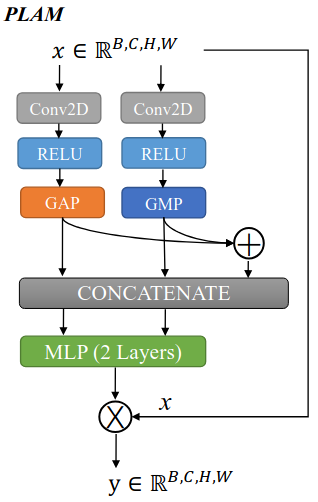
\includegraphics[height=0.7\textheight]{images/plam.png}
        \caption{Mô-đun PLAM.}
    \end{figure}

\end{frame}

\begin{frame}{\secname: \subsecname: PLAM}
    Trong kiến trúc LViT, nhánh Transformer có ưu điểm trong việc học các quan hệ toàn cục giữa các vùng ảnh thông qua cơ chế self-attention. Tuy nhiên, do tập trung vào tương tác toàn cục, Transformer có thể làm suy giảm một số chi tiết cục bộ quan trọng như biên tổn thương, kết cấu nhỏ hoặc sự thay đổi cường độ tại các vùng hẹp. Đây là những thông tin có vai trò quan trọng trong phân đoạn ảnh y khoa, đặc biệt khi vùng bệnh lý có kích thước nhỏ hoặc ranh giới không rõ ràng.

    \bigskip
    PLAM được đưa vào để bù đắp hạn chế này bằng cách kết hợp thông tin từ nhiều nhánh đặc trưng khác nhau. Global Average Pooling giúp mô hình nắm bắt xu hướng tổng quát của toàn bộ bản đồ đặc trưng, trong khi Global Max Pooling nhấn mạnh các đặc điểm mạnh nhất, thường tương ứng với những vùng có tín hiệu nổi bật hoặc đặc trưng phân biệt cao. Việc sử dụng đồng thời hai phép pooling giúp PLAM thu được cả thông tin ngữ cảnh tổng quát lẫn các dấu hiệu cục bộ quan trọng.
\end{frame}

\subsection{Hàm mất mát}
\begin{frame}{\secname: \subsecname}
Trong mô hình LViT, hàm mất mát (loss function) được thiết kế khác nhau tùy thuộc vào việc dữ liệu đang được huấn luyện là dữ liệu có nhãn (học giám sát) hay dữ liệu không có nhãn (học bán giám sát):
    \begin{itemize}
        \item Đối với dữ liệu có nhãn (Supervised): Mô hình sử dụng trung bình cộng của hai hàm mất mát cơ bản là Dice loss ($L_{Dice}$) và Cross-Entropy ($L_{CE}$).
        $$L_{Sup} = \frac{1}{2}(L_{Dice} + L_{CE})$$
        \item Đối với dữ liệu không có nhãn (Unsupervised): Mô hình sử dụng hàm mất mát tương tự như trên nhưng cộng thêm một thành phần hàm mất mát đặc biệt có tên là Language Vision Loss.
        $$L_{Sup} = \frac{1}{2}(L_{Dice} + L_{CE}) + \alpha L_{LV}$$
    \end{itemize}
\end{frame}

\begin{frame}{\secname: \subsecname: LV Loss}
    \begin{align*}
        TextSim = \frac{x_{text, p} \cdot x_{text, c}}{|x_{text, p}||x_{text, c}|}
    \end{align*}
    
    \textbf{Tìm độ tương đồng văn bản (TextSim):} Với mỗi ảnh không nhãn, đầu vào vẫn đi kèm một đoạn chú thích bệnh mô tả. Sau khi mô hình sinh ra nhãn giả cho ảnh này, đoạn chú thích tương ứng được mã hóa thành vector đặc trưng văn bản $x_{text,p}$. Mô hình so sánh vector này với các vector đặc trưng văn bản của những mẫu có nhãn, ký hiệu là $x_{text,c}$. Mẫu có văn bản đối chiếu gần nhất về mặt ngữ nghĩa được xem là mẫu tham chiếu phù hợp nhất.
    
\end{frame}

\begin{frame}{\secname: \subsecname: LV Loss}
    \begin{align*}
        ImgSim = \frac{x_{img, p} \cdot x_{img, c}}{|x_{img, p}||x_{img, c}|} \\
        L_{LV} = 1 - ImgSim \\
    \end{align*}
    
    \textbf{Tìm độ tương đồng hình ảnh (ImgSim):} Sau khi xác định được nhãn đối chiếu từ bước TextSim, mô hình tiếp tục so sánh đặc trưng hình ảnh của nhãn giả với đặc trưng hình ảnh của nhãn đối chiếu. Cụ thể, vector đặc trưng của vùng dự đoán từ ảnh không nhãn được ký hiệu là $x_{img,p}$, còn vector đặc trưng của vùng đối chiếu từ ảnh có nhãn được ký hiệu là $x_{img,c}$. Độ tương đồng cosine giữa hai vector này cho biết nhãn giả có gần với nhãn đối chiếu hay không trong không gian đặc trưng hình ảnh.
\end{frame}

\begin{frame}{\secname: \subsecname: LV Loss}
    Mục đích của LV loss là tận dụng trực tiếp thông tin từ văn bản y tế để tạo thêm tín hiệu giám sát cho các ảnh không có nhãn.
    
    \bigskip
    Thay vì chỉ tin vào mặt nạ do mô hình tự dự đoán, LV loss sử dụng chú thích văn bản để tìm một mẫu có nhãn mang ý nghĩa gần nhất, rồi dùng mẫu đó như một điểm neo tham chiếu. Vì các cơ quan và tổn thương trên ảnh y tế thường có vị trí giải phẫu tương đối ổn định, sự tương đồng giữa các mô tả văn bản có thể cung cấp gợi ý hữu ích về vị trí phân đoạn.
    
    \bigskip
    Nhờ vậy, LV loss giúp hạn chế trường hợp mô hình dự đoán mặt nạ lệch khỏi vùng cơ quan hoặc vùng bệnh lý mà văn bản đang mô tả, đồng thời làm cho nhãn giả nhất quán hơn với tri thức ngữ nghĩa từ chú thích y khoa.
\end{frame}

\subsection{Cơ chế sinh nhãn giả}

\begin{frame}{\secname: \subsecname}

Với các ảnh không nhãn, mô hình không có mặt nạ chuẩn để tính trực tiếp các hàm mất mát phân đoạn như Dice loss và Cross-Entropy. Vì vậy, cần có một cơ chế sinh nhãn giả nhằm tạo ra các mặt nạ tạm thời cho dữ liệu không nhãn.

\bigskip
Tuy nhiên, nhãn giả do mô hình tự dự đoán thường không ổn định, đặc biệt ở các giai đoạn đầu của quá trình huấn luyện. Nếu sử dụng trực tiếp dự đoán ở một vòng huấn luyện duy nhất, mặt nạ có thể bị nhiễu, bị lệch khỏi vùng tổn thương hoặc thay đổi mạnh giữa các vòng lặp. Điều này có thể khiến mô hình học theo các nhãn sai và làm giảm chất lượng phân đoạn.

\end{frame}


\begin{frame}{\secname: \subsecname}
    Giả định:
    
    Trong $n$ vòng huấn luyện gần nhất, các trọng số của mô hình thực chất chỉ đang dao động xung quanh một điểm tối ưu thực sự. Kéo theo đó, mask dự đoán cho ảnh A ở vòng 10, vòng 11, vòng 12... cũng đang dao động qua lại quanh ranh giới phân vùng chuẩn xác của vùng bệnh lý. 

    \bigskip
    Nếu chỉ lấy dự đoán của vòng hiện tại, mask có thể bị lệch hoặc nhiễu. Nhưng khi "đúc kết" kết quả dự đoán của tất cả các vòng trước đó trên chính bức ảnh A, các sai số dao động sẽ tự triệt tiêu lẫn nhau, tạo ra một mask nhãn giả (pseudo label) mượt mà, ổn định và có độ tin cậy cao hơn rất nhiều để dẫn dắt mô hình học tập.

\end{frame}
\begin{frame}{\secname: \subsecname}
    Đối với dữ liệu không có nhãn:
    \begin{enumerate}
        \item \textbf{Dự đoán mặt nạ hiện tại:} Ở vòng huấn luyện $t$, mô hình nhận ảnh không nhãn làm đầu vào và sinh ra bản đồ xác suất hiện tại $P_{current}$.

        \item \textbf{Kết hợp với nhãn giả trước đó:} Dự đoán hiện tại được kết hợp với nhãn giả đã tích lũy từ vòng trước thông qua cơ chế EMA:
        \[
            P_t = \beta P_{t-1} + (1 - \beta) P_{current}
        \]
        Trong đó, $P_t$ là nhãn giả được cập nhật tại vòng huấn luyện $t$, $P_{t-1}$ là nhãn giả ở vòng trước, $P_{current}$ là dự đoán hiện tại của mô hình và $\beta$ là hệ số làm mượt.

        \item \textbf{Sử dụng nhãn giả để huấn luyện:} Nhãn giả $P_t$ sau khi cập nhật được dùng như mặt nạ tham chiếu tạm thời để tính các thành phần mất mát phân đoạn cho ảnh không nhãn, chẳng hạn Dice loss và Cross-Entropy. Nhờ đó, dữ liệu không nhãn vẫn có thể đóng góp vào quá trình tối ưu mô hình.
    \end{enumerate}
\end{frame}

% \begin{frame}{\secname: \subsecname}
%     \begin{enumerate}
%         \setcounter{enumi}{\value{saveenumi}}
%         \item So sánh với nhãn đối chiếu thông qua LV Loss: Hệ thống sẽ đem vector đặc trưng của câu text hiện tại đi so sánh với các câu text có trong kho dữ liệu, tìm ra một câu text có độ tương đồng cao nhất. Khi tìm thấy, nó sẽ "mượn" Mask có sẵn tương ứng với câu text đó để làm Nhãn đối chiếu. Sau đó tính toán LV Loss. \\
%         Mục tiêu là giám sát vị trí phân đoạn, đảm bảo mask tạo ra phải nằm đúng vị trí cơ quan giải phẫu mà văn bản đang mô tả, tránh việc dự đoán sai lệch hoàn toàn.
%     \end{enumerate}
% \end{frame}

\subsection{Pipeline huấn luyện và sử dụng}
\begin{frame}{\secname: \subsecname}
    \begin{figure}[H]
        \centering
        \begin{minipage}{0.48\textwidth}
            \centering
            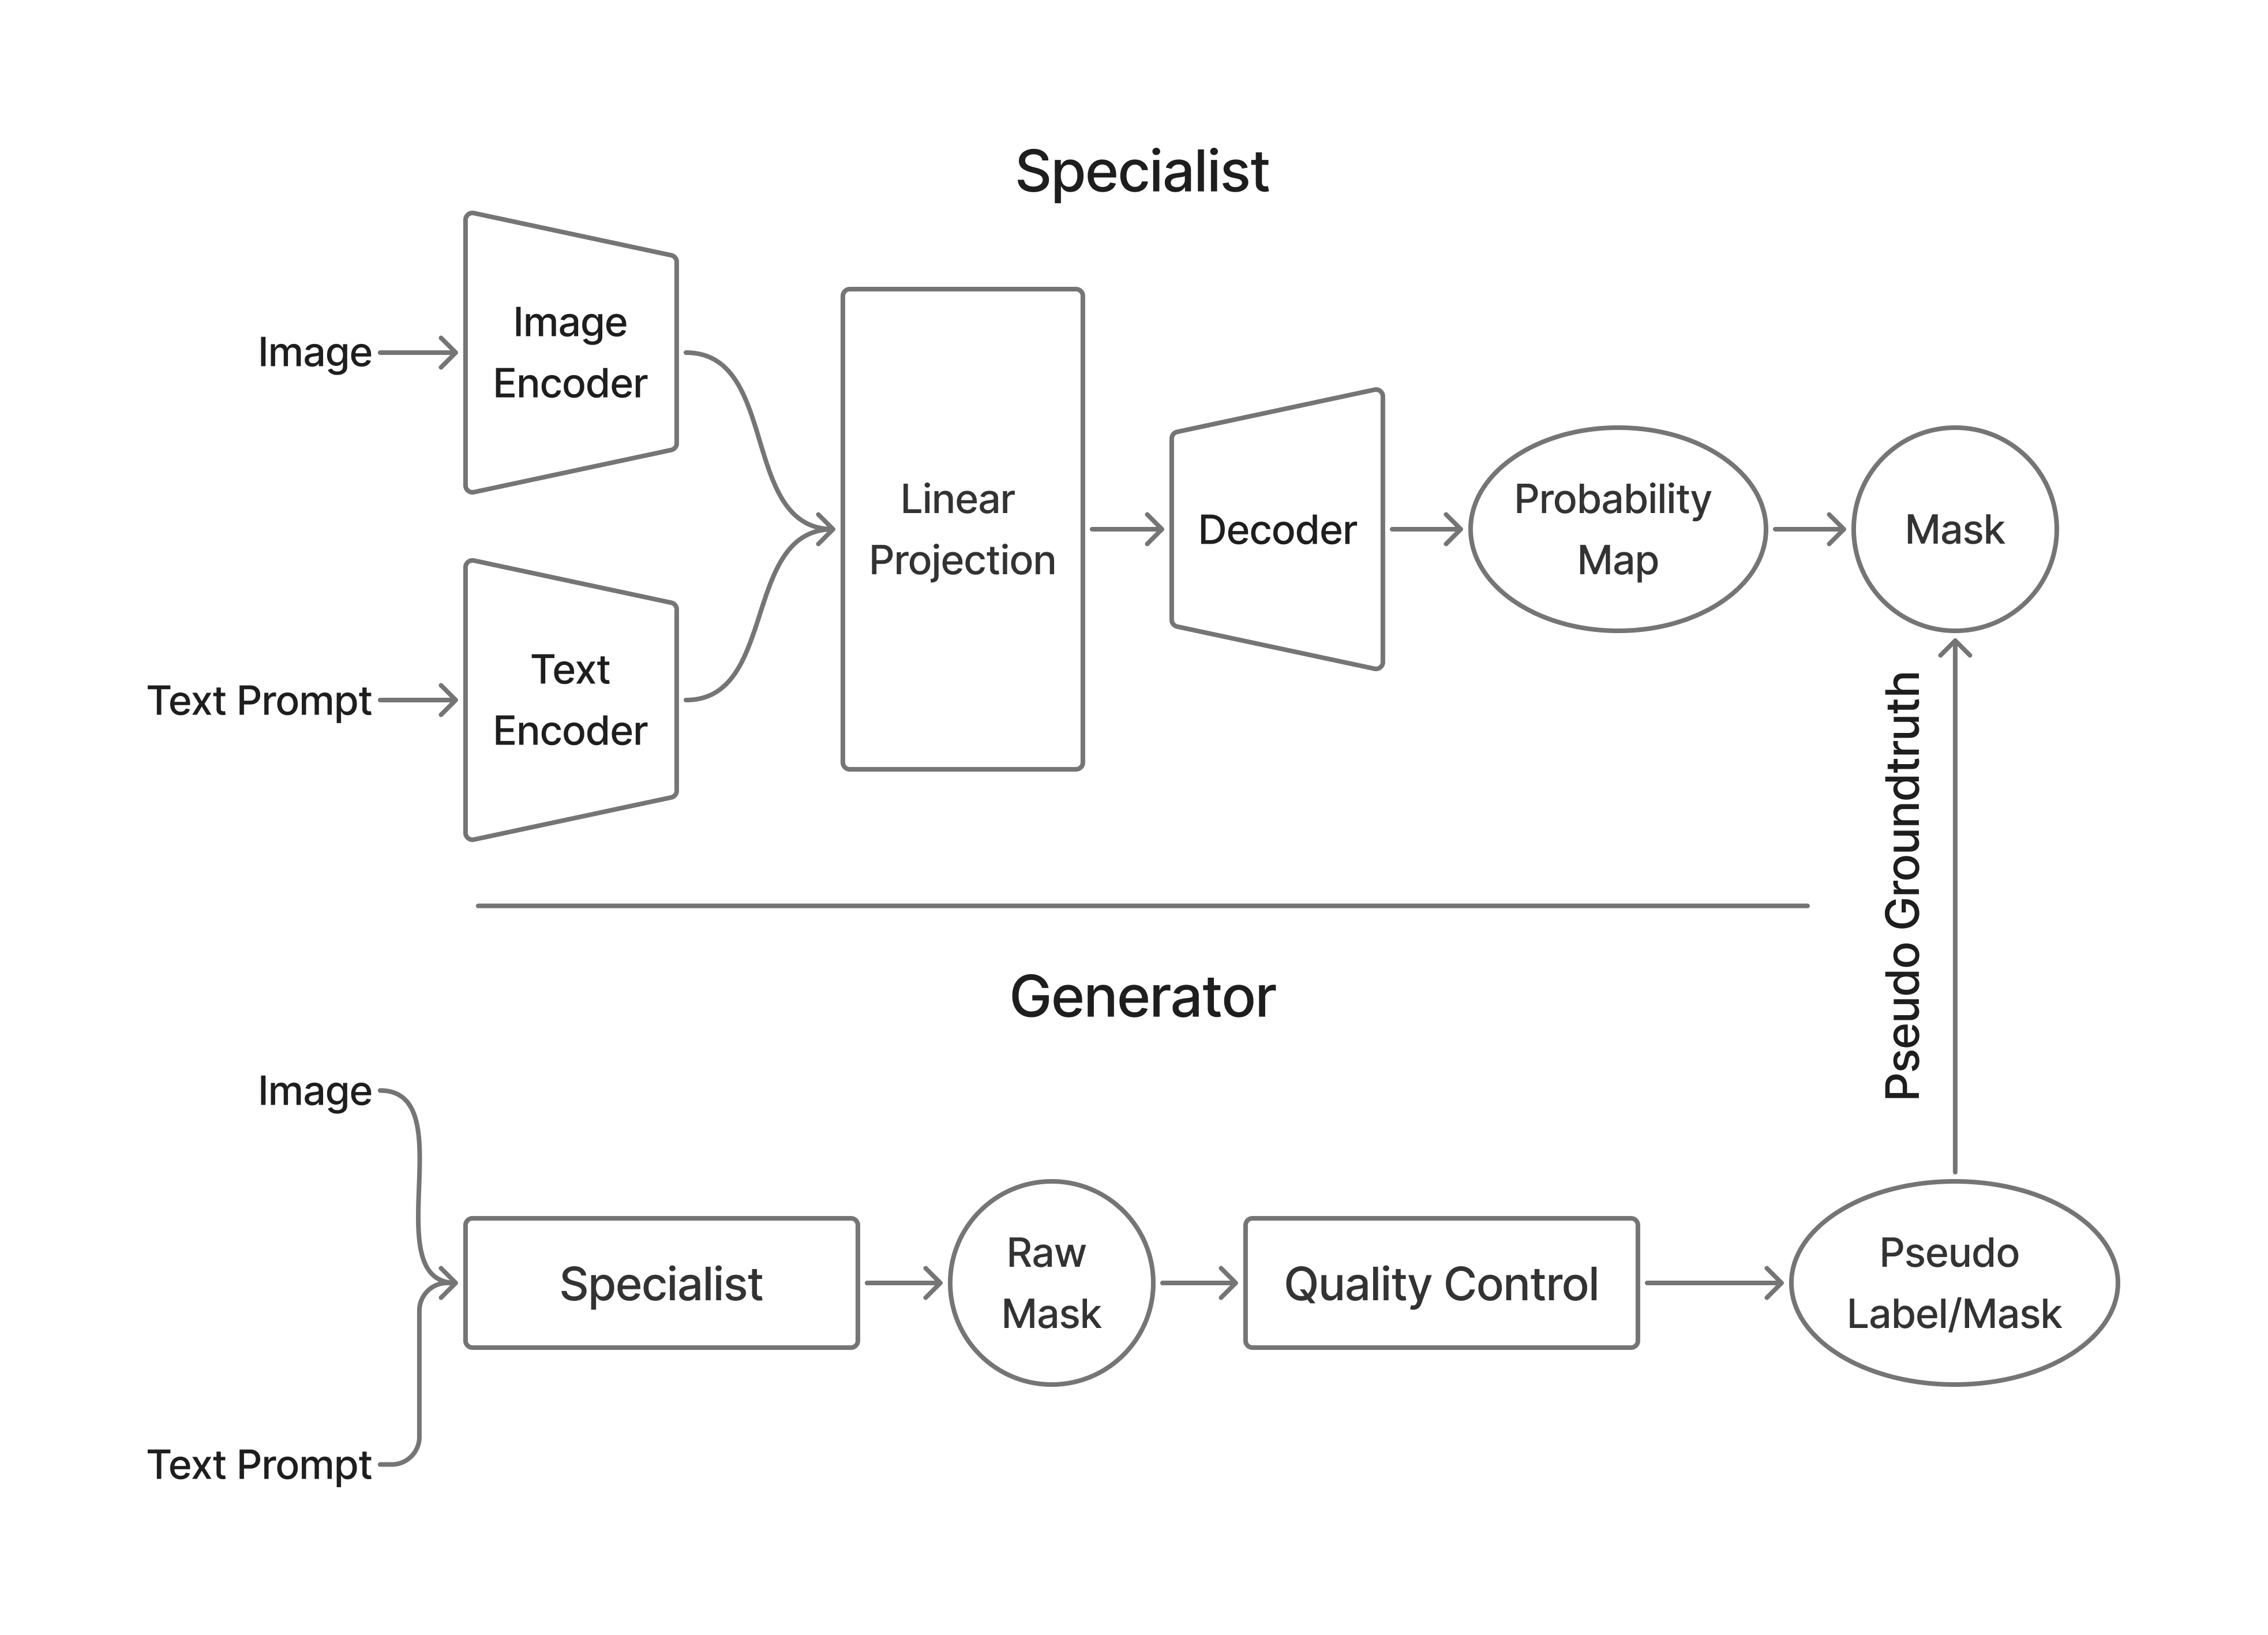
\includegraphics[width=\linewidth]{images/offline-pipeline.png}
            \caption{Pipeline huấn luyện mô hình}
            \label{fig:offline}
        \end{minipage}
        \hfill
        \begin{minipage}{0.48\textwidth}
            \centering
            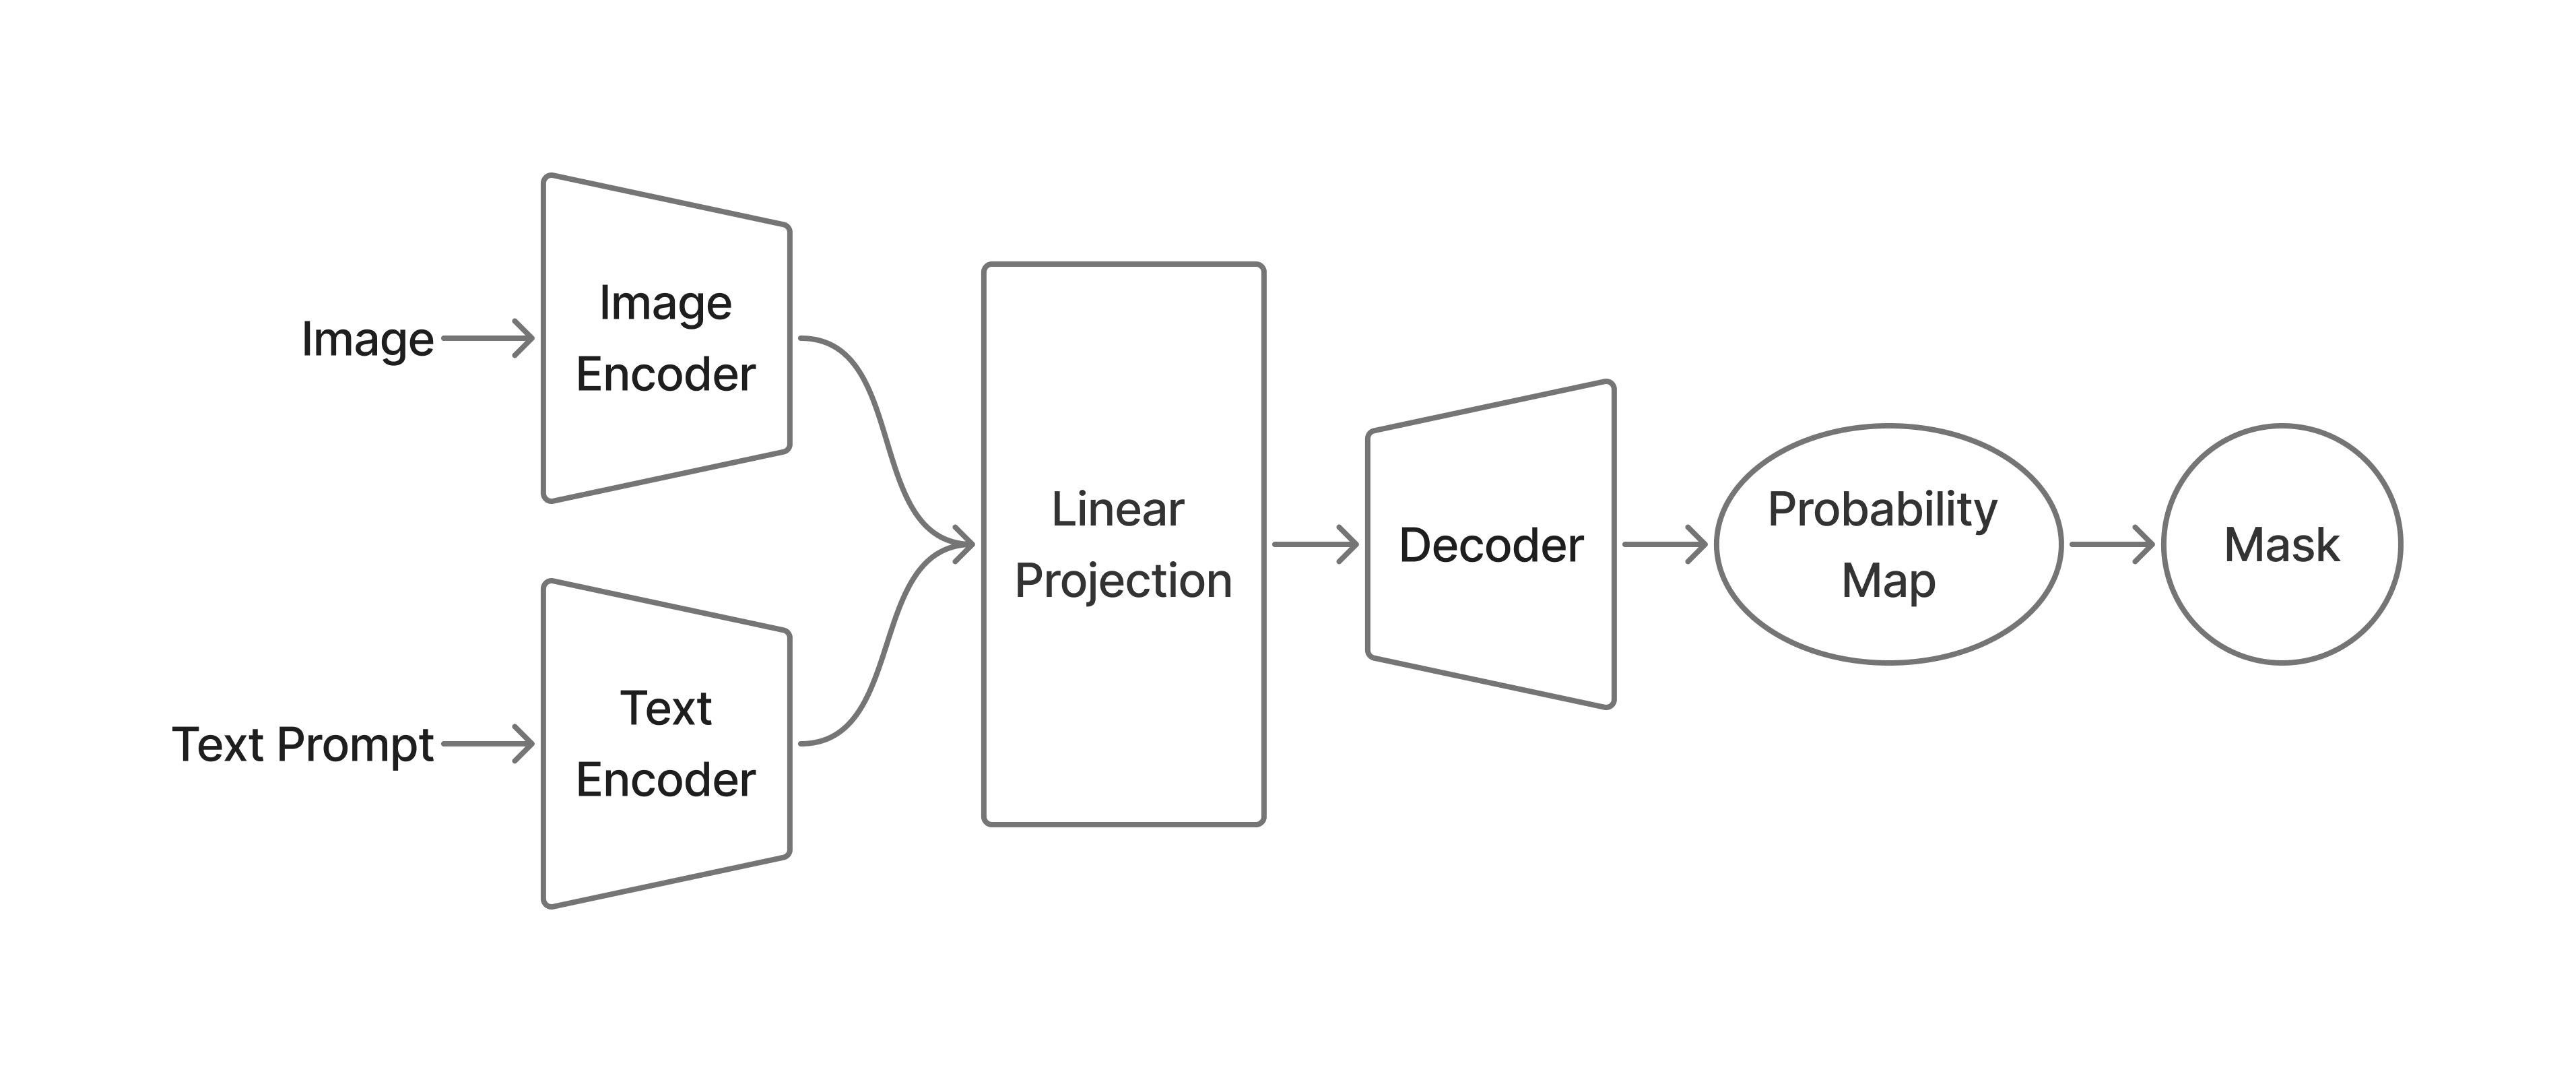
\includegraphics[width=\linewidth]{images/online-pipeline.png}
            \caption{Pipeline sử dụng mô hình}
            \label{fig:online}
        \end{minipage}
    \end{figure}
\end{frame}

\begin{frame}{\secname: \subsecname}

    Hình \ref{fig:offline} mô tả pipeline huấn luyện mô hình ở chế độ ngoại tuyến. Trong giai đoạn này, hệ thống sử dụng cả dữ liệu có nhãn và dữ liệu không nhãn. Đối với dữ liệu có nhãn, mặt nạ chuẩn được dùng trực tiếp. Đối với dữ liệu không nhãn, mô hình cần thêm cơ chế sinh nhãn giả để tạo ra mặt nạ tạm thời phục vụ quá trình huấn luyện.

    \bigskip
    Pipeline này gồm hai thành phần quan trọng: \textit{Specialist} và \textit{Generator}. Specialist chịu trách nhiệm sinh mặt nạ phân đoạn ban đầu dựa trên ảnh đầu vào và câu nhắc văn bản, trong khi Generator tổng hợp và cập nhật các nhãn giả ổn định hơn từ các dự đoán qua nhiều vòng huấn luyện.
\end{frame}

\begin{frame}{\secname: \subsecname}

    Hình \ref{fig:online} mô tả pipeline sử dụng mô hình trong thực tế sau khi quá trình huấn luyện đã hoàn tất. Ở giai đoạn suy luận, người dùng cung cấp một ảnh y khoa và một câu nhắc văn bản mô tả vùng cần phân đoạn. Hai nguồn đặc trưng này được kết hợp trong mô hình để sinh ra bản đồ xác suất phân đoạn. Sau đó, bản đồ xác suất được xử lý bằng một ngưỡng quyết định để tạo ra mặt nạ nhị phân cuối cùng. Mặt nạ này biểu diễn vùng tổn thương hoặc cơ quan phù hợp với nội dung câu nhắc đầu vào.

    \bigskip
    Điểm quan trọng của pipeline online là mô hình có tính linh hoạt theo câu nhắc. Cùng một ảnh đầu vào có thể tạo ra các mặt nạ khác nhau nếu người dùng thay đổi mô tả văn bản.
\end{frame}

\begin{frame}{\secname: \subsecname}
    \begin{figure}[H]
        \centering
        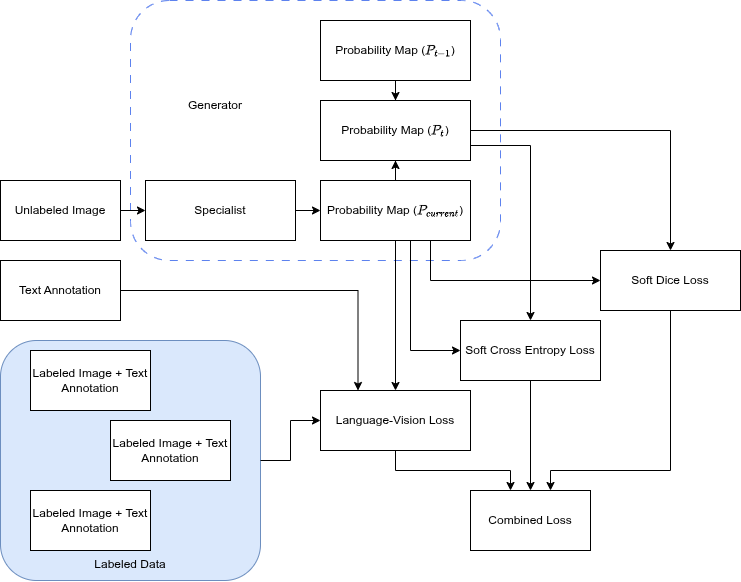
\includegraphics[width=0.6\textwidth]{images/lvit_loss_calculation.png}
        \caption{Pipeline tính toán hàm mất mát và xây dựng nhãn giả chi tiết}
        \label{fig:loss_calculation}
    \end{figure}
\end{frame}

\begin{frame}{\secname: \subsecname}
    Hình \ref{fig:loss_calculation} mô tả chi tiết quá trình xây dựng nhãn giả và tính toán hàm mất mát cho ảnh không nhãn. Trước hết, mô hình nhận ảnh không nhãn cùng câu nhắc văn bản tương ứng để sinh ra bản đồ xác suất hiện tại $P_{current}$. Mỗi phần tử trong $P_{current}$ biểu diễn xác suất pixel tương ứng thuộc về vùng cần phân đoạn, thay vì chỉ đưa ra quyết định nhị phân là nền hoặc tổn thương. Do đó, $P_{current}$ không chỉ cho biết vị trí vùng dự đoán mà còn thể hiện mức độ tự tin của mô hình tại từng điểm ảnh.

    \bigskip
    Điểm quan trọng là các hàm mất mát trong bước này được áp dụng theo hướng \textit{soft}. Điều này có nghĩa là mục tiêu huấn luyện không bắt buộc phải là mặt nạ nhị phân chỉ gồm các giá trị 0 và 1, mà có thể là một bản đồ xác suất với các giá trị thực nằm trong khoảng từ 0 đến 1. Ví dụ, một pixel có giá trị 0.8 trong nhãn giả thể hiện rằng pixel đó có khả năng cao thuộc vùng tổn thương, trong khi giá trị 0.4 thể hiện mức độ không chắc chắn lớn hơn. Cách biểu diễn này giữ lại nhiều thông tin hơn so với việc gán cứng pixel đó thành 0 hoặc 1.
\end{frame}